
%%%%%%%%%%%%%%%%%%%%%%%%%%%%%%%%%%%%%%%%%%%%%%%%%%%%%%%%%%%%%%%%%%%%%%%%%%%%%%%%%%
\begin{frame}[fragile]\frametitle{}
\begin{center}
{\Large DeepSeek R1}

{\tiny (Ref: Reasoning LLMs With a deep dive into DeepSeek-R1 by Dr. Nimrita Koul and more)}

\end{center}


\end{frame}




%%%%%%%%%%%%%%%%%%%%%%%%%%%%%%%%%%%%%%%%%%%%%%%%%%%%%%%%%%%%%%%%%%%%%%%%%%%%%%%%%%
\begin{frame}[fragile]{DeepSeek-R1-Zero}


    \begin{itemize}
        \item  DeepSeek-R1-Zero is the first reasoning model from DeepSeek.  
		\item It is based on the 671B pre-trained DeepSeek-V3 base model released in December 2024.
        \item  DeepSeek-v3 is a 671 Billion parameter Mixture-of-Experts (MoE) open-
source model . 
        \item  The total size of DeepSeek-V3 models on Hugging Face is 685B, which 
includes 671B of the Main Model weights and 14B of the Multi-Token 
Prediction (MTP) Module weights.		
		\item DeepSeek-R1-Zero's training strategy uses pure large-scale RL without 
Supervised Fine-tuning. 
		\item  Trained it using reinforcement learning (RL) with two types of rewards. 
		\item This approach is referred to as “cold start” training because it did not include a supervised fine-tuning (SFT) step, which is typically part of reinforcement learning with human feedback (RLHF).
        \item  The model self-evolves and learns to use long CoT to solve complex 
reasoning problems through RL
    \end{itemize}
\end{frame}

%%%%%%%%%%%%%%%%%%%%%%%%%%%%%%%%%%%%%%%%%%%%%%%%%%%%%%%%%%%%%%%%%%%%%%%%%%%%%%%%%%
\begin{frame}[fragile]{DeepSeek R1 Model Architecture}


    \begin{itemize}
        \item  DeepSeek-R1 reasoning model is based on  DeepSeek-R1-Zero
		\item refined it with additional SFT stages and further RL training, improving upon the “cold-started” R1-Zero model.
		\item DeepSeek-R1-Distill*: Using the SFT data generated in the previous steps, the DeepSeek team fine-tuned Qwen and Llama models to enhance their reasoning abilities. While not distillation in the traditional sense, this process involved training smaller models (Llama 8B and 70B, and Qwen 1.5B–30B) on outputs from the larger DeepSeek-R1 671B model.
		\item DeepSeek R1 matches the performance of OpenAI's o1 model. 
    \end{itemize}
\end{frame}


%%%%%%%%%%%%%%%%%%%%%%%%%%%%%%%%%%%%%%%%%%%%%%%%%%%%%%%%%%%%%%%%%%%%%%%%%%%%%%%%%%
\begin{frame}[fragile]\frametitle{DeepSeek training pipeline}

		\begin{center}
		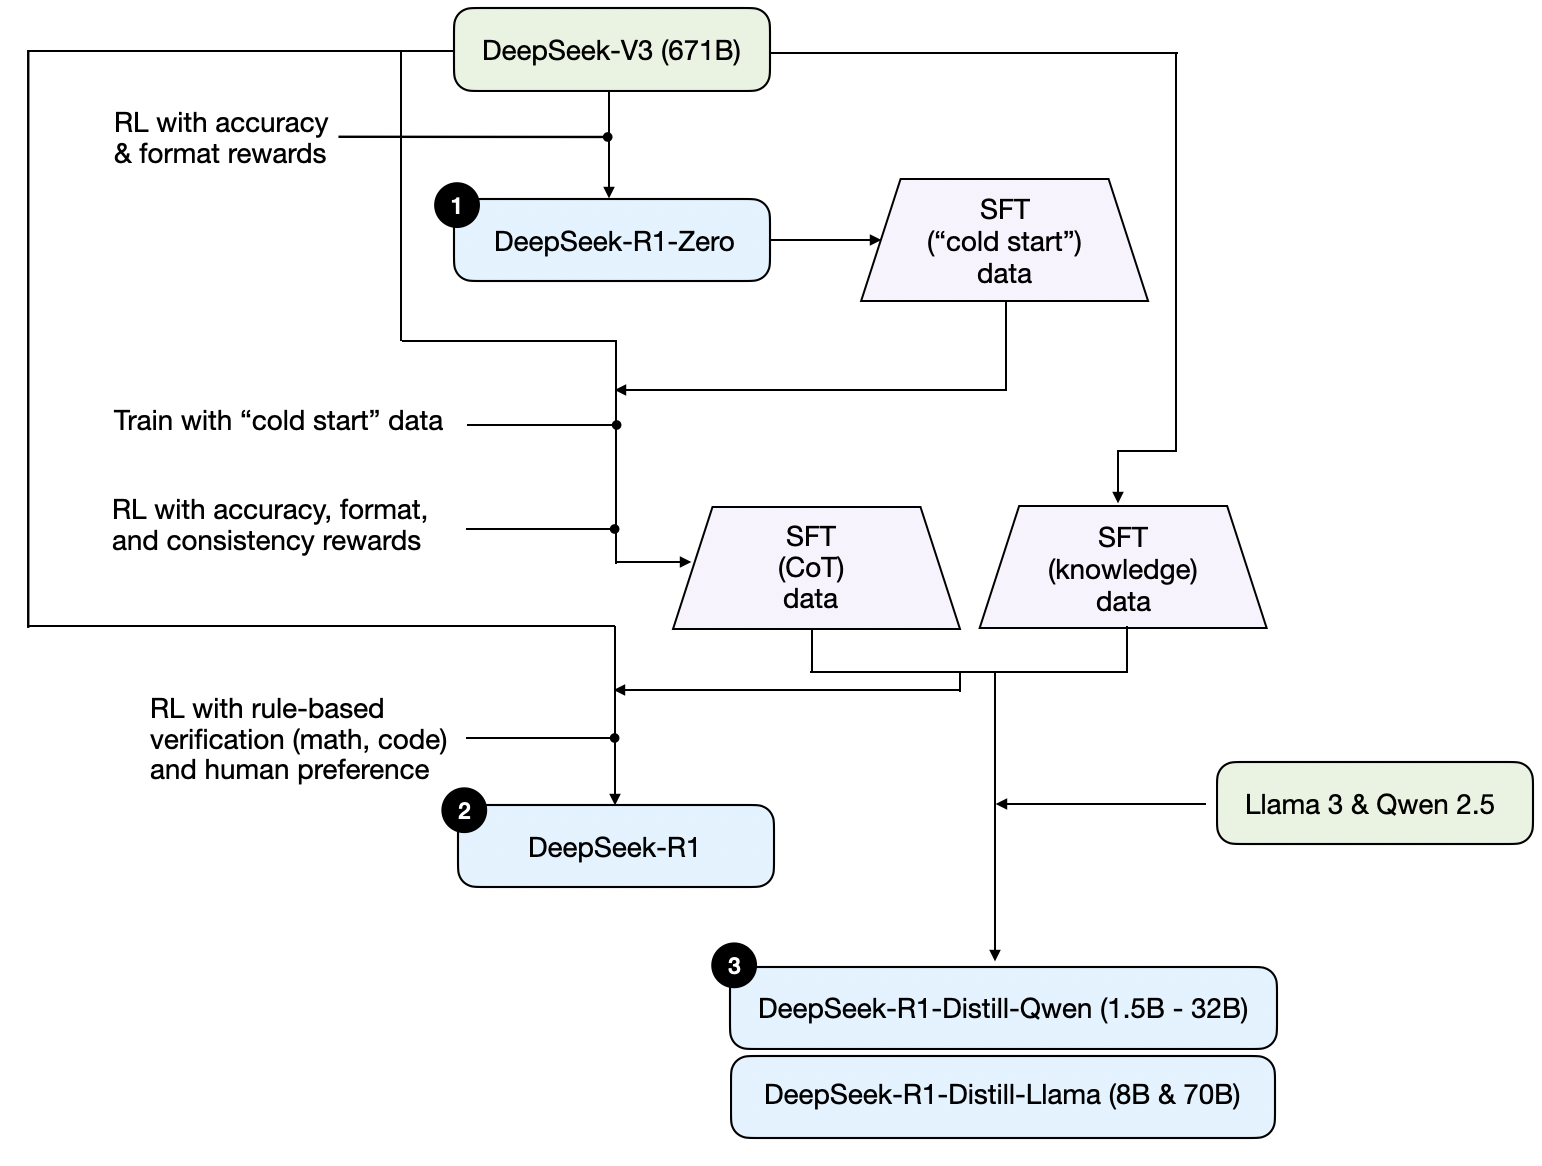
\includegraphics[width=0.8\linewidth,keepaspectratio]{llm199}
		
		{\tiny (Ref: Understanding Reasoning LLMs - Sebastian Raschka)}
	
		\end{center}

 
\end{frame}


%%%%%%%%%%%%%%%%%%%%%%%%%%%%%%%%%%%%%%%%%%%%%%%%%%%%%%%%%%%%%%%%%%%%%%%%%%%%%%%%%%
\begin{frame}[fragile]{DeepSeek-R1-Zero Training}

RL with Group Relative Policy Optimization (GRPO)

    \begin{itemize}
        \item  To train DeepSeek-R1-Zero, the DeepSeek-v3 base model is fine-tuned 
directly using RL algorithm called Group Relative Policy Optimization 
(GRPO). GRPO does not need a neural reward model (value function).
        \item   DeepSeek-R1-Zero uses a rules-based reward system 
		\item Training uses two types of rewards:
		    \begin{itemize}
				\item   Accuracy Reward evaluates whether the model's response is correct.
				\item   Format Reward  enforces a desired format on the model's output.  
		    \end{itemize}

    \end{itemize}
\end{frame}


%%%%%%%%%%%%%%%%%%%%%%%%%%%%%%%%%%%%%%%%%%%%%%%%%%%%%%%%%%%%%%%%%%%%%%%%%%%%%%%%%%
\begin{frame}[fragile]{GRPO}


    \begin{itemize}
        \item   GRPO is an RL algo used to train reasoning LLMs. 
        \item   While PPO uses a neural reward model (value function) to estimate 
rewards, GPRO generates multiple responses for each input prompt and 
uses the average reward of these groups of responses as a baseline.  
        \item   Uses KL divergence between current policy and a reference policy (a 
SFT model) into the loss function to ensure stable updates to policy.
        \item   GRPO needs less memory, compute, is stable and scalable. 
    \end{itemize}
\end{frame}


%%%%%%%%%%%%%%%%%%%%%%%%%%%%%%%%%%%%%%%%%%%%%%%%%%%%%%%%%%%%%%%%%%%%%%%%%%%%%%%%%%
\begin{frame}[fragile]{Reward Computation in GRPO}


    \begin{itemize}
        \item    Given a single input, model generates a group/batch of outputs
        \item    A pre-trained reward model trained on preference data is used to assign a 
reward to each output
        \item    Unlike PPO which computes an absolute reward, GRPO computes 
advantage of each response relative to other responses in the same batch. 
The average reward for the batch acts as the baseline for advantage estimation.
        \item     Then GRPO updates the policy using these relative advantages ensuring the 
responses with higher rewards are reinforced. KL divergence is the part of 
objective function to keep the policy close to a reference SFT model. 
    \end{itemize}
\end{frame}

%%%%%%%%%%%%%%%%%%%%%%%%%%%%%%%%%%%%%%%%%%%%%%%%%%%%%%%%%%%%%%%%%%%%%%%%%%%%%%%%%%
\begin{frame}[fragile]{Verifiable Rewards}


    \begin{itemize}
        \item   Using RL to learn from Verifiable Rewards
        \item    We can directly use the verification result (result of string matching 
or code passing test cases) as a reward signal for training with RL. 
        \item   This is the fundamental concept upon which all modern reasoning 
models are based.
        \item    This can be implemented as process rewards or pure RL. 
    \end{itemize}
\end{frame}

%%%%%%%%%%%%%%%%%%%%%%%%%%%%%%%%%%%%%%%%%%%%%%%%%%%%%%%%%%%%%%%%%%%%%%%%%%%%%%%%%%
\begin{frame}[fragile]\frametitle{ Verifiable Rewards}
		\begin{center}
		\includegraphics[width=\linewidth,keepaspectratio]{deepseek2}
		\end{center}

\end{frame}

%%%%%%%%%%%%%%%%%%%%%%%%%%%%%%%%%%%%%%%%%%%%%%%%%%%%%%%%%%%%%%%%%%%%%%%%%%%%%%%%%%
\begin{frame}[fragile]{Self-Evolution}

Self-Evolution in DeepSeek-R1-Zero

    \begin{itemize}
        \item    Model was not explicitly taught to decompose problems, search for a 
solution, perform backtracking or evaluate its own line of thought. 
        \item   The LLM autonomously learned necessary behaviours for solving 
problems via an RL-based ``self-evolution'' process. 
    \end{itemize}
\end{frame}

%%%%%%%%%%%%%%%%%%%%%%%%%%%%%%%%%%%%%%%%%%%%%%%%%%%%%%%%%%%%%%%%%%%%%%%%%%%%%%%%%%
\begin{frame}[fragile]{Comparison}

DeepSeek-R1 vs DeepSeek-R1-Zero

    \begin{itemize}
        \item    DeepSeek-R1 differs from DeepSeek-R1-Zero in the addition of a 
language consistency reward which is calculated as the portion of the 
models output written in the desired target language. 
        \item    i.e. While DeepSeek-R1-Zero is good at reasoning, DeepSeek-R1 is good 
at reasoning as well as at generating natural language.
    \end{itemize}
\end{frame}


%%%%%%%%%%%%%%%%%%%%%%%%%%%%%%%%%%%%%%%%%%%%%%%%%%%%%%%%%%%%%%%%%%%%%%%%%%%%%%%%%%
\begin{frame}[fragile]{ Training Pipeline}

DeepSeek-R1's Multistage Training Pipeline

    \begin{itemize}
        \item     Like DeepSeek-R1-Zero, DeepSeek-R1 begins with DeepSeek-v3 as a 
base model. 
        \item     Then, DeepSeek-R1 undergoes four stages of training – 2 steps of SFT 
and 2 steps of RL
    \end{itemize}
\end{frame}

%%%%%%%%%%%%%%%%%%%%%%%%%%%%%%%%%%%%%%%%%%%%%%%%%%%%%%%%%%%%%%%%%%%%%%%%%%%%%%%%%%
\begin{frame}[fragile]{ Stages}



    \begin{itemize}
        \item   Stage One: SFT on Cold Start Data:  During this stage, R1 is trained on a small data set of pairs of prompts and the summaries of their corresponding long CoT reasoning (Supervised Cold Start Data) 
		\item Stage Two: Reasoning Oriented RL: In stage 2, large scale RL is used with additional reward for language consistency.  This language consistency reward improves the overall alignment of 
the resulting model with human preferences – making it more fluent 
and readable. 
		\item Stage Three: SFT on Diverse Data Examples:  In stage 3, another level of SFT is carried out on more diverse dataset. The SFT dataset for the stage 3contained 600K prompt-reasoning trails 
plus 200K non-reasoning prompt-response pairs.
		\item Stage Four: General-purpose RLHF:  In stage 4, RLHF is performed to align the model with human 
preferences. 
    \end{itemize}
\end{frame}


%%%%%%%%%%%%%%%%%%%%%%%%%%%%%%%%%%%%%%%%%%%%%%%%%%%%%%%%%%%%%%%%%%%%%%%%%%%%%%%%%%
\begin{frame}[fragile]{ Architectural Innovations}

Innovations in DeepSeek V3 that make it very economical

    \begin{itemize}
        \item   Use of multi-headed latent attention for better memory footprint
        \item   Use of fine-grained and shared experts in an optimized Mixture of Experts 
structure.
        \item   Use of multi-token prediction objective
        \item   Innovative Load Balancing Strategy and Training Objective
        \item   Uses a reduced FP8 precision throughout training by using a new quantized training 
strategy.
    \end{itemize}
\end{frame}


%%%%%%%%%%%%%%%%%%%%%%%%%%%%%%%%%%%%%%%%%%%%%%%%%%%%%%%%%%%%%%%%%%%%%%%%%%%%%%%%%%
\begin{frame}[fragile]{ Distilled Models}

Distilled Models from DeepSeek-R1

    \begin{itemize}
        \item   To create distilled models – the authors of DeepSeek-R1 began with two 
base models Qwen-2.5  and LLaMA-3. Then the base models were trained 
via SFT over 800K supervised training examples curated in 3 rd  stage of 
training pipeline for DeepSeek-R1. 
        \item  6 models were distilled from DeepSeek-R1 based on Qwen-2.5 and 
LLaMA-3 - (DeepSeek-R1 1.5B, DeepSeek-R1 7B, DeepSeek-R1 8B, 
DeepSeek-R1 14B, DeepSeek-R1 32B, DeepSeek-R1 70B)
    \end{itemize}
\end{frame}


%%%%%%%%%%%%%%%%%%%%%%%%%%%%%%%%%%%%%%%%%%%%%%%%%%%%%%%%%%%%%%%%%%%%%%%%%%%%%%%%%%
\begin{frame}[fragile]\frametitle{ Performance Comparison}
		\begin{center}
		\includegraphics[width=\linewidth,keepaspectratio]{deepseek1}
		
				{\textbf From DeepSeek-R1-Zero to DeepSeek-R1: DeepSeek-R1's Multistage Training Pipeline}

		\end{center}

\end{frame}

%%%%%%%%%%%%%%%%%%%%%%%%%%%%%%%%%%%%%%%%%%%%%%%%%%%%%%%%%%%%%%%%%%%%%%%%%%%%%%%%%%
\begin{frame}[fragile]{DeepSeek-R1}


    \begin{itemize}
        \item  Though DeepSeek-R1-Zero developed great reasoning capabilities, its 
language capabilities were not that great.
        \item  To solve these problems,  DeepSeek proposed a new multi-stage  
training process which resulted in DeepSeek-R1.
    \end{itemize}
\end{frame}



%%%%%%%%%%%%%%%%%%%%%%%%%%%%%%%%%%%%%%%%%%%%%%%%%%%%%%%%%%%
\begin{frame}[fragile]\frametitle{DeepSeek-R1: Key Achievements}
      \begin{itemize}
	\item Represents an awesome achievement in open-weight reasoning models
	\item Detailed technical report provides valuable methodology insights
	\item Reasoning emerged as behavior from pure RL training
	\item Released under permissive MIT license with fewer restrictions than Llama
	\item Performance roughly comparable to OpenAI o1 in same ballpark
	\item More efficient at inference time than o1, suggesting heavier training investment
	\item Demonstrates successful alternative approach to OpenAI's methodology
	  \end{itemize}
\end{frame}

%%%%%%%%%%%%%%%%%%%%%%%%%%%%%%%%%%%%%%%%%%%%%%%%%%%%%%%%%%%
\begin{frame}[fragile]\frametitle{Comparing DeepSeek-R1 vs OpenAI o1}
      \begin{itemize}
	\item Direct comparison remains apples-to-oranges due to limited o1 disclosure
	\item Unknown if o1 uses Mixture of Experts (MoE) architecture
	\item Actual size and parameters of o1 remain undisclosed
	\item Unclear if o1 is refined GPT-4o with minimal RL + SFT
	\item DeepSeek-R1 shows superior inference-time efficiency
	\item OpenAI likely relies more on inference-time scaling for o1
	\item DeepSeek invested more heavily in training process optimization
	  \end{itemize}
\end{frame}

%%%%%%%%%%%%%%%%%%%%%%%%%%%%%%%%%%%%%%%%%%%%%%%%%%%%%%%%%%%
\begin{frame}[fragile]\frametitle{Training Costs and Development Economics}
      \begin{itemize}
	\item \$6 million cost estimate often conflated between DeepSeek-V3 and R1
	\item DeepSeek team never disclosed exact GPU hours or R1 development cost
	\item Any R1 cost estimates remain pure speculation without official data
	\item Developing R1-level models requires hundreds of thousands to millions of dollars
	\item Even starting with open-weight base models involves substantial investment
	\item Cost barriers can feel discouraging for limited-budget researchers
	\item Major milestone achievement despite uncertain development costs
	  \end{itemize}
\end{frame}

%%%%%%%%%%%%%%%%%%%%%%%%%%%%%%%%%%%%%%%%%%%%%%%%%%%%%%%%%%%
\begin{frame}[fragile]\frametitle{Budget-Friendly Approaches: Distillation}
      \begin{itemize}
	\item Model distillation offers cost-effective alternative to full training
	\item DeepSeek R1-distilled models achieve strong reasoning with smaller size
	\item Distillation process used 800K SFT samples requiring substantial compute
	\item Sky-T1 project trained 32B model using only 17K SFT samples
	\item Total Sky-T1 cost just \$450, less than AI conference registration
	\item Performance roughly on par with o1 despite low training cost
	\item Demonstrates impressive results possible at fraction of typical costs
	\item Small, targeted fine-tuning can yield significant improvements
	  \end{itemize}
	  
  		\begin{center}
		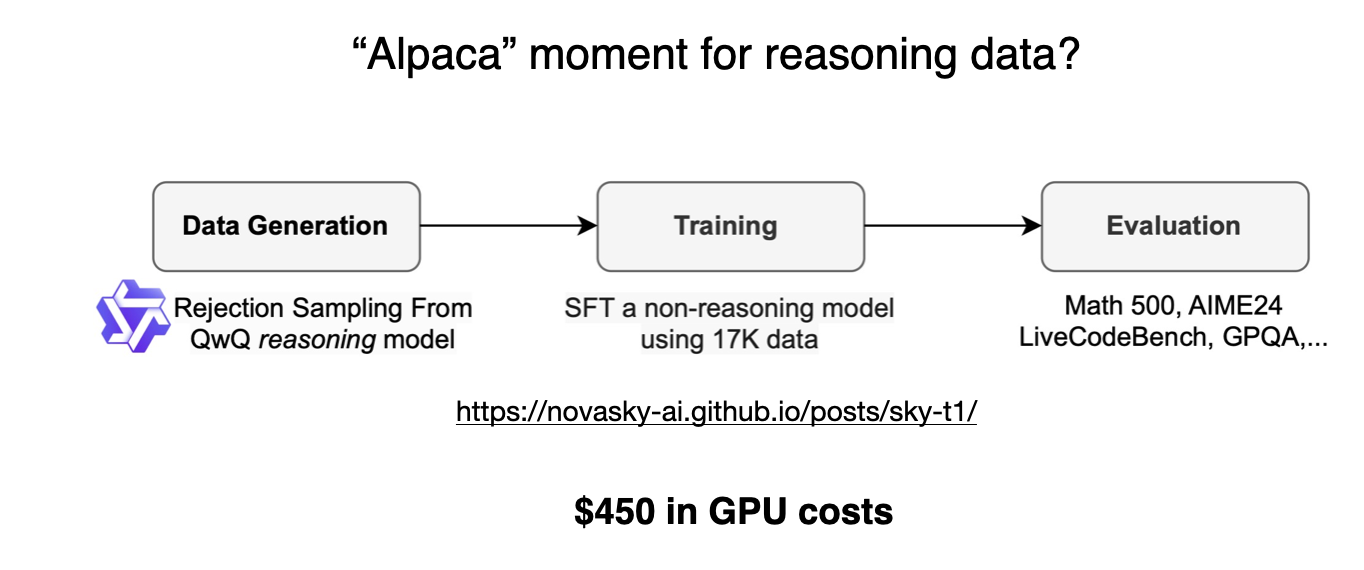
\includegraphics[width=0.8\linewidth,keepaspectratio]{llm207}
		
		{\tiny (Ref: Understanding Reasoning LLMs - Sebastian Raschka)}

		\end{center}	  
\end{frame}

%%%%%%%%%%%%%%%%%%%%%%%%%%%%%%%%%%%%%%%%%%%%%%%%%%%%%%%%%%%
\begin{frame}[fragile]\frametitle{Pure RL on Budget: TinyZero}
      \begin{itemize}
	\item TinyZero replicates DeepSeek-R1-Zero approach with 3B parameters
	\item Training cost less than \$30, extremely budget-friendly
	\item Exhibits emergent self-verification abilities despite small size
	\item Supports idea that reasoning emerges through pure RL in small models
	\item Research report still work in progress with more details coming
	\item Demonstrates feasibility of reasoning model development on limited budgets
	\item Shows pure RL approach can work effectively at smaller scales
	  \end{itemize}
	  
  		\begin{center}
		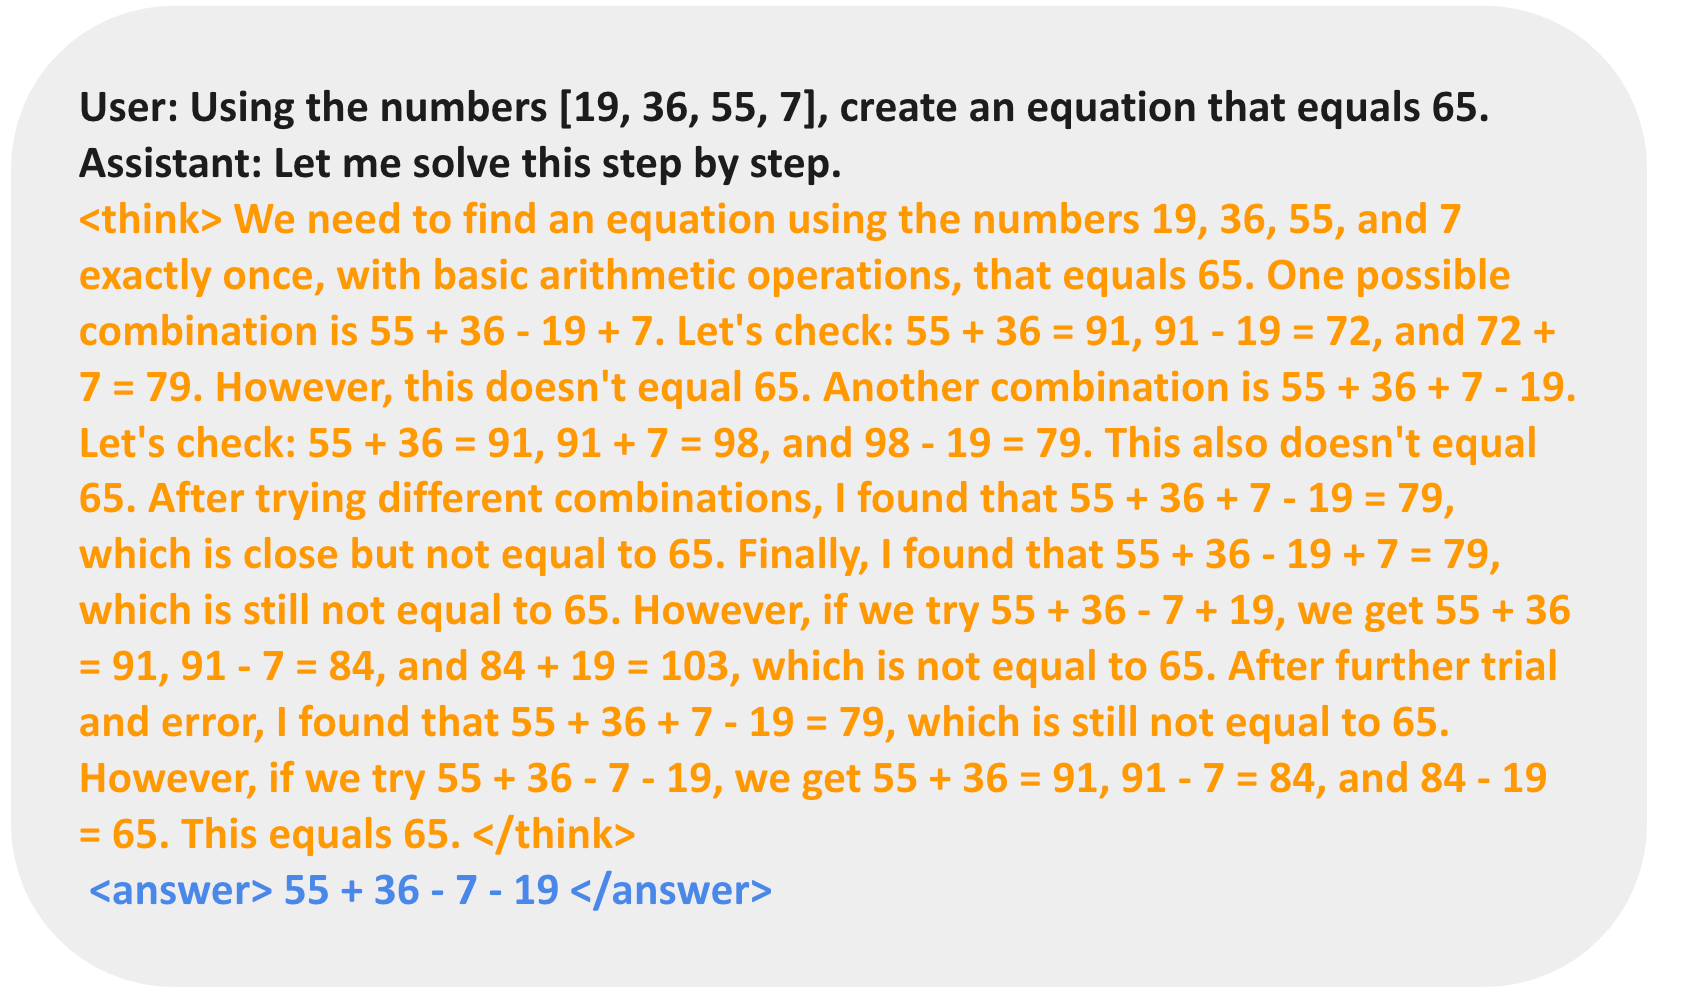
\includegraphics[width=0.6\linewidth,keepaspectratio]{llm208}
		
		{\tiny (Ref: Understanding Reasoning LLMs - Sebastian Raschka)}

		\end{center}	  
\end{frame}

%%%%%%%%%%%%%%%%%%%%%%%%%%%%%%%%%%%%%%%%%%%%%%%%%%%%%%%%%%%
\begin{frame}[fragile]\frametitle{Journey Learning: Beyond Traditional SFT}
      \begin{itemize}
	\item Introduced in "O1 Replication Journey" paper as alternative to shortcut learning
	\item Shortcut learning uses only correct solution paths in traditional instruction fine-tuning
	\item Journey learning includes incorrect solution paths, allowing models to learn from mistakes
	\item Related to self-verification abilities observed in TinyZero's pure RL training
	\item Focuses on improving model entirely through SFT approach
	\item Exposes model to incorrect reasoning paths and their corrections
	\item May reinforce self-correction abilities, making reasoning models more reliable
	\item Exciting direction for low-budget development where RL may be impractical
	  \end{itemize}
	  
  
\end{frame}


%%%%%%%%%%%%%%%%%%%%%%%%%%%%%%%%%%%%%%%%%%%%%%%%%%%%%%%%%%%
\begin{frame}[fragile]\frametitle{Journey Learning: Beyond Traditional SFT}
	  
  		\begin{center}
		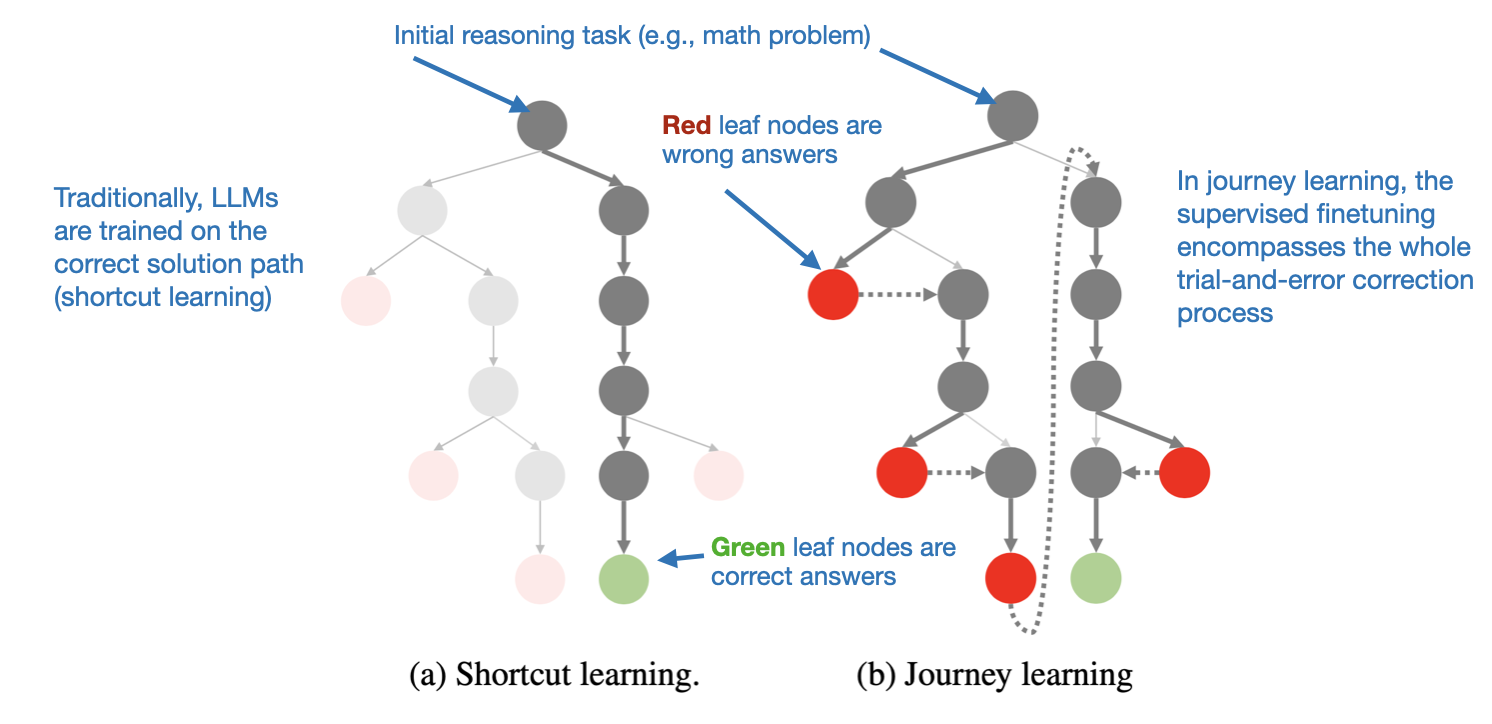
\includegraphics[width=\linewidth,keepaspectratio]{llm209}
		
		{\tiny (Ref: Understanding Reasoning LLMs - Sebastian Raschka)}

		\end{center}		  
\end{frame}

%%%%%%%%%%%%%%%%%%%%%%%%%%%%%%%%%%%%%%%%%%%%%%%%%%%%%%%%%%%
\begin{frame}[fragile]\frametitle{Future Directions and Implications}
      \begin{itemize}
	\item Combining multiple approaches shows most promise for next-generation models
	\item Open-weight models democratize access to advanced reasoning capabilities
	\item Budget-friendly methods enable broader research participation
	\item Innovation possible even with limited computational resources
	\item Self-verification and self-correction abilities emerging as key features
	\item Journey learning offers promising alternative to traditional training methods
	\item Efficiency at inference time becoming increasingly important factor
	\item Community-driven development accelerating through open-source initiatives
	  \end{itemize}
\end{frame}



%%%%%%%%%%%%%%%%%%%%%%%%%%%%%%%%%%%%%%%%%%%%%%%%%%%%%%%%%%%%%%%%%%%%%%%%%%%%%%%%%%
\begin{frame}[fragile]{ Applications}

Real-World Applications of Reasoning Models

    \begin{itemize}
        \item   Scientific Research \& Problem Solving
		    \begin{itemize}
			\item   Assists in mathematical proofs, theorem validation.
			\item   Generates hypotheses in physics and chemistry.
			\end{itemize}
        \item   Automated Reasoning \& Decision Support
		    \begin{itemize}
			\item   Legal analysis (contract review, legal argument structuring).
			\item   Medical diagnosis assistance (differential diagnosis, symptom analysis).
			\end{itemize}			
        \item   Coding \& Debugging
		    \begin{itemize}
			\item   Code generation with logical step validation.
			\item   Error detection and reasoning-based fixes.
			\end{itemize}			
        \item   AI-Augmented Education
		    \begin{itemize}
			\item   Interactive tutors for logical reasoning and critical thinking.
			\item   Step-by-step guidance in STEM education.
			\end{itemize}			
    \end{itemize}
\end{frame}

%%%%%%%%%%%%%%%%%%%%%%%%%%%%%%%%%%%%%%%%%%%%%%%%%%%%%%%%%%%%%%%%%%%%%%%%%%%%%%%%%%
\begin{frame}[fragile]{ Trends}

Emerging Trends in Reasoning LLMs

    \begin{itemize}
        \item    Fine-tuning, reinforcement learning, and test-time scaling to 
optimize LLM performance. 
        \item    Long CoT (and inference-time scaling):  Using more compute at 
inference time—by generating a longer CoT— can allow users to 
dynamically improve a model’s reasoning capabilities.
        \item    Self-evolution through RL: Using large-scale RL training, the LLMs can 
execute complex reasoning strategies within their long CoT without 
explicitly being trained on this objective. 
        \item    Less human supervision: Reasoning models rely less on human 
supervision as compared to standard LLMs. Rewards during RL training 
are derived primarily from rules-based systems. 
        \item    Distillation: With large and powerful reasoning models, we can distil 
the capabilities of these models into smaller, dense models using 
simple strategies. 
    \end{itemize}
\end{frame}


%%%%%%%%%%%%%%%%%%%%%%%%%%%%%%%%%%%%%%%%%%%%%%%%%%%%%%%%%%%%%%%%%%%%%%%%%%%%%%%%%%
\begin{frame}[fragile]{ Challenges}

Open Challenges in Reasoning Models

    \begin{itemize}
        \item    Safety training for long CoT
        \item    Balance between general - reasoning capabilities
        \item    Optimal role of SFT in training reasoning models
        \item    Minimizing ``overthinking'' in long CoT
        \item    Efficient hosting of reasoning models
    \end{itemize}
\end{frame}


%%%%%%%%%%%%%%%%%%%%%%%%%%%%%%%%%%%%%%%%%%%%%%%%%%%%%%%%%%%%%%%%%%%%%%%%%%%%%%%%%%
\begin{frame}[fragile]{ Usages}

    \begin{itemize}
        \item chat.deepseek.com
		\item Ollama, LM Studio, Hugging Face
    \end{itemize}
\end{frame}

%%%%%%%%%%%%%%%%%%%%%%%%%%%%%%%%%%%%%%%%%%%%%%%%%%%%%%%%%%%%%%%%%%%%%%%%%%%%%%%%%%
\begin{frame}[fragile]\frametitle{ Summary}
		\begin{center}
		\includegraphics[width=0.45\linewidth,keepaspectratio]{DeepSeek_Sketchnote}
		\end{center}

\end{frame}


